\documentclass[11pt,a4paper,notitlepage,twocolumn]{article}
\usepackage{fullpage}
\usepackage[utf8x]{inputenc}
\usepackage{ucs}
\usepackage{amsmath}
\usepackage{amsfonts}
\usepackage{amssymb}
\usepackage{ifpdf}
\usepackage{float}
\ifpdf
\usepackage[pdftex]{graphicx}
\graphicspath{{./img/}}
\DeclareGraphicsExtensions{.pdf}
\else
\usepackage[dvips]{graphicx}
\graphicspath{{./img/}}
\DeclareGraphicsExtensions{.eps}
\fi

\renewcommand{\figurename}{Obr.}

\begin{document}

\title{\textbf{Astrofyzika 2011 LS}\\vypracování otázek k zápočtovámu testu}
\author{Peter Boráros}
\date{10.5.2011}

\maketitle

\paragraph{Co je astronomická jednotka?}
Jednotka dlžky. Približná stredná vzdialenosť Zeme od Slnka. Skratka je \textbf{AU}.
 $ 1AU \approx 149~597~870 700 m. $
\paragraph{Co je světelný rok? }
Jednotka dlžky. Vzdialenpsť, ktorú uletí svetlo v vákuu za 1 rok.Skratka je \textbf{ly}.
$ 1ly \approx 10^{16} m $.
\paragraph{Jak je definován parsek?}
Jednotka dlžky. Je to vzdialenosť Slnka od objektu, ktorý má paralaktický uhol rovný
jednej uhlovej sekunde (\textbf{p}arallax of one \textbf{ar}c\textbf{sec}ond). 
Skratka je \textbf{pc}.
$ 1pc \approx 3,1\cdot 10^{16} m $.
\paragraph{Co je paralaxa?}
Paralaxa je úhel, který svírají přímky vedené ze dvou různých míst v prostoru k pozorovanému
bodu. Jako paralaxa se také označuje zdánlivý rozdíl polohy bodu vzhledem k pozadí při
pozorování ze dvou různých míst.
\paragraph{Jak vzdálená je nejbližší hvězda od Slunce?}
Je to Proxima Centauri a je od Slnka vzdialená $ 4,22ly $ t.j. $ 1,3pc $ 
alebo $ 43\cdot10^{12} $
\paragraph{Co vyjadřuje Planckův vyzařovací zákon?}
Planckův vyzařovací zákon vyjadřuje závislost intenzity záření I absolutně černého 
tělesa na frekvenci $ \omega $.
\[  dI = \frac{\hbar}{\pi^2c^2} \frac{\omega^3}{e^{\frac{\hbar \omega}{kT}-1}}d\omega  \]
kde\\
$ \omega $ je uhlová frekvence záření,\\
$ I $ je intenzita záření,\\
$ T $ je teplota absolutně černého tělesa,\\
$ \hbar $ je redukovaná Planckova konstanta,\\
$ c $ je rychlost světla ve vakuu a\\
$ k $ Boltzmannova konstanta.
\paragraph{Jak zní Wienův posunovací zákon?}
Wienův posunovací zákon je fyzikální zákon, který konstatuje, že v záření absolutně černého tělesa je maximální energie vyzařována na vlnové délce, která se s rostoucí termodynamickou teplotou snižuje (tj. čím teplejší je těleso, tím vyzařuje na kratších vlnových délkách, tj. vyšších frekvencích):
\[ \lambda_{max} = \frac{b}{T} \]
kde\\
$ \lambda_{max}  $ je vlnová délka maxima vyzařování,\\
$ T $ je teplota tělesa a 
$ b $ je tzv. Wienova konstanta, jejíž hodnota je přibližně $ b = 2,898 mm\cdot K. $.

Spektrální hustota záření v tomto maximu je přitom úměrná páté mocnině teploty, 
$ W_\lambda \propto T^5 $.
\paragraph{Jak zní Stefanův-Boltzmannův zákon?}
Stefanův-Boltzmannův zákon publikovaný roku 1879 Ludwigem Boltzmannem a Josefem Stefanem popisuje celkovou intenzitu záření absolutně černého tělesa. Tento zákon říká, že intenzita vyzařování roste se čtvrtou mocninou termodynamické teploty zářícího tělesa.
\[ I = \sigma T^4 \]
kde\\
$ I $ celková intenzita zá\v{r}ení (podíl výkonu a plochy) $ [W\cdot m^{-2}] $,\\
$ \sigma $ je Stefanova-Boltzmannova konstanta 
$ \sigma = 5,670400 \cdot 10^{-8} W m^{-2} K^{-4}  $\\
$ T $ je termodinamická teplota.
\paragraph{Na čem závisí vizuální jasnost hvězdy?}
Závisí na hustote svetelného toku dopadajúceho na oko pozorovateľa z danej hviezdy.
\paragraph{Jaká je zhruba povrchová teplota Slunce?}
Povrchová teplota Slnka je približne $ 5780K $
\paragraph{Jak je definována (relativní) magnituda?}
Hvězdná velikost (zdánlivá magnituda, zdánlivá hvězdná velikost, zdánlivá jasnost, symbol
$ mag $ nebo $ ^m $) je fotometrická veličina používaná v astronomii, 
která udává jasnost objektu (světelného zdroje) na obloze.
Její hodnota představuje zdánlivou, tedy subjektivně vnímanou nebo přístrojem detekovanou,
jasnost hvězdy.

Magnituda je logaritmická jednotka, u které platí, že 1 $ mag $ rozdílu jasnosti odpovídá
jasnostem v poměru $ 2,512:1 $ (tzv. Pogsonův poměr). Tento poměr byl zvolen tak, že hvězdy
lišící se o 5 mag mají vzájemný poměr jasností 1:100, čímž se zhruba dodržuje starověký 
význam magnitudy. Je třeba upozornit, že v souladu s tímto historickým významem znamená 
vyšší magnituda nižší jasnost hvězdy.

Rozdíl hvězdných velikostí dvou hvězd $ m_1 − m_2 $ je tedy definován pomocí tzv.
Pogsonovy rovnice
\[ m_1 − m_2 = −2,5 log_{10}(I_1/I_2) \]
kde $ I_1 $ a $ I_2 $ jsou hustoty světelného toku (množství světla dopadajících na jednotku
plochy za jednotku času) dopadajícího na lidské oko nebo čidlo přístroje ze dvou srovnávaných
hvězd. Hvězdná velikost m libovolné hvězdy je tedy rovna
$ m = −2,5 log_{10}(I/I_0) $
kde $ I_0 $ je hustota světelného toku hvězdy, které byla definitoricky přiřčena hvězdná
velikost $ 0^m $. Původně byly hvězdné velikosti kalibrovány podle vybraných hvězd v okolí
severního světového pólu (tzv. severní polární posloupnost).
\paragraph{Jak je definována absolutní magnituda?}
Absolutní hvězdná velikost (absolutní jasnost, absolutní magnituda) je veličina určující
hvězdnou velikost vztaženou na standardní pozorovací podmínky.
U hvězd a objektů podobných hvězdám označujeme tuto veličinu symbolem $ M $ a definujeme
ji jako hvězdnou velikost, jakou by tato hvězda měla při pozorování ze vzdálenosti 
$ 10pc $ čili $ 32,6ly $. Vztah mezi absolutní hvězdnou velikostí $ M $ a zdánlivou 
hvězdnou velikostí m je dán rovnicí
\[ M = m + 5 [1 − log_{10}(d)] \]
kde\\
$ d $ je vzdálenost hvězdy v parsecích od pozorovatele (od Země).

\paragraph{Co je Hertzsprungův-Russelův diagram?}
\begin{figure}[H]
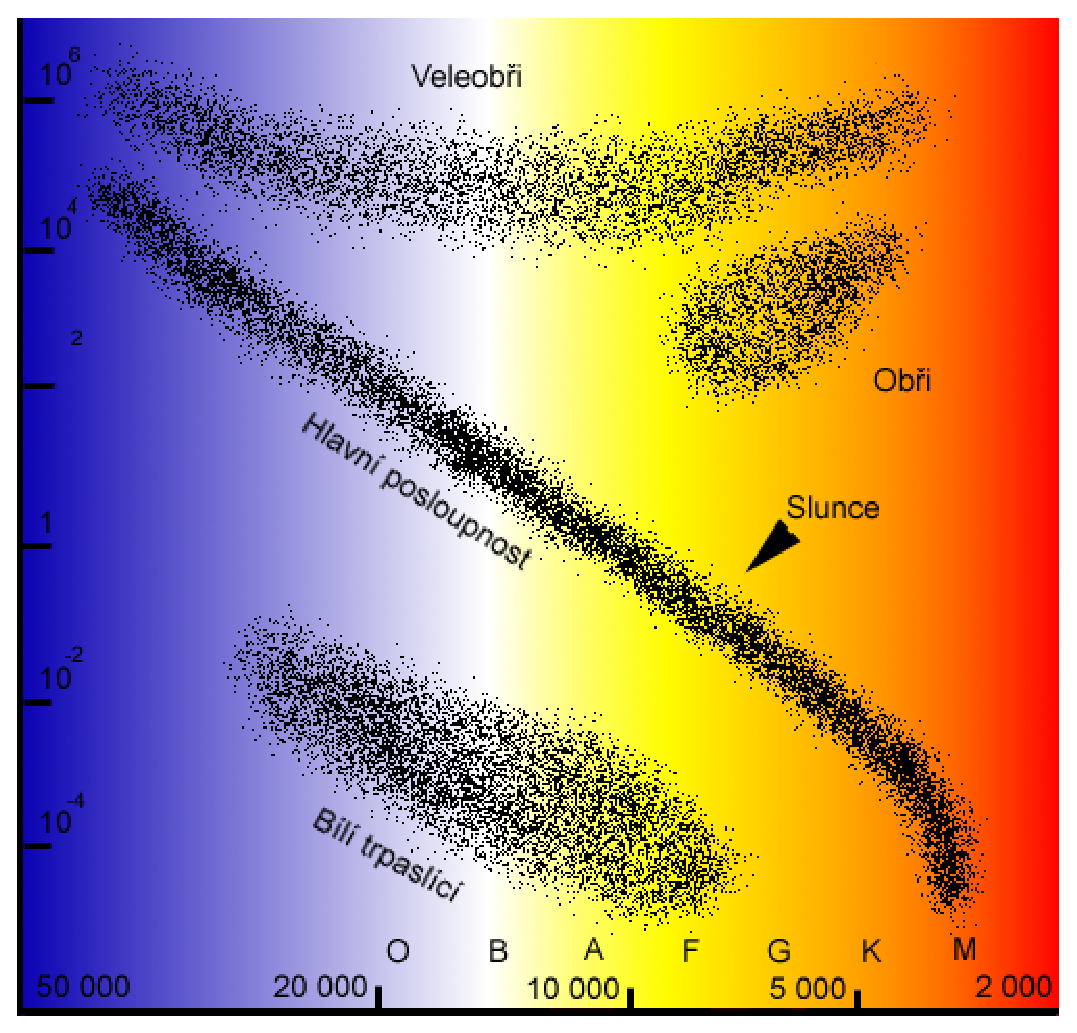
\includegraphics[width=0.5\textwidth]{HR_diagram}
\caption{HR diagram}
\label{fig:HR_diagram}
\end{figure}
Hertzsprungův-Russellův diagram vyjadřuje závislost povrchové teploty (spektrální typ)
hvězd 
na~jejích svítivosti (zářivý výkon) nebo absolutní magnitudě v různých fázích vývoje. 
Závislost absolutní hvězdné velikosti na spektrární třídě hvězd objevil v roce 1909 E.
Hertzsprungem a později zdokonalené H. N. Russellem. Obr. \ref{fig:HR_diagram}.
\paragraph{Co jsou to kuželosečky?}
\begin{figure}[H]
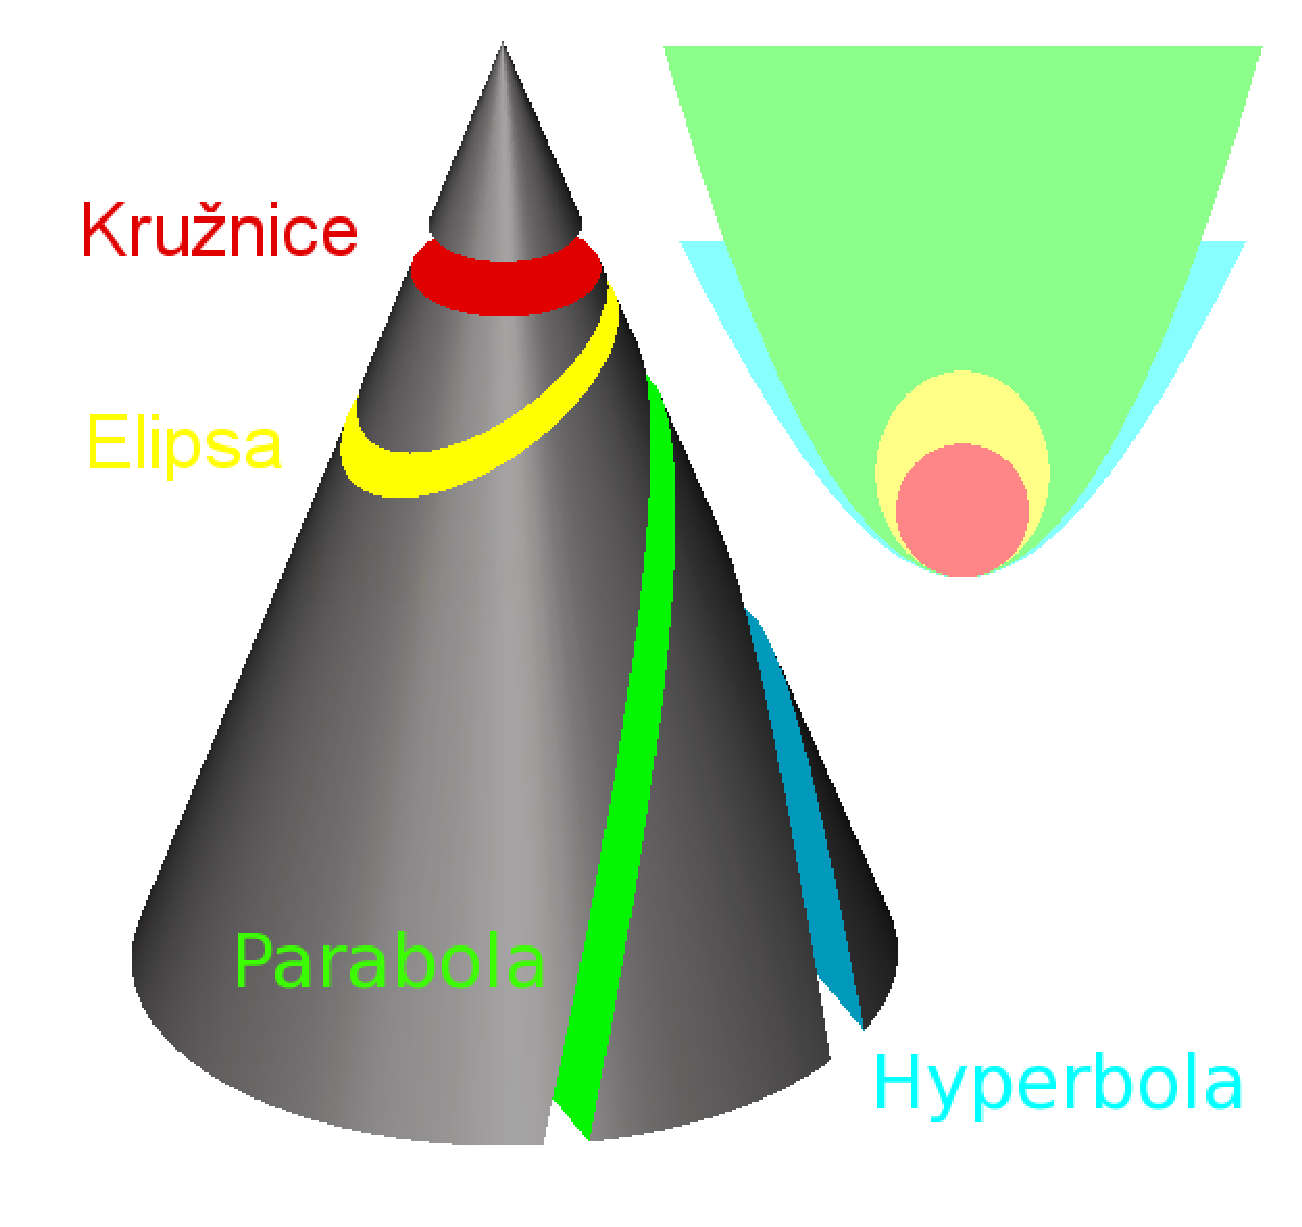
\includegraphics[width=0.38\textwidth]{kuzelosecky}
\caption{Kuželosečky}
\label{fig:kuzelosecky}
\end{figure}
Kuželosečka je rovinná křivka, která vznikne jako průnik roviny s pláštěm rotačního kuželu
(tzv. kuželová plocha), přičemž rovina neprochází jeho vrcholem. Obr. \ref{fig:kuzelosecky}.
\paragraph{Po jakých trajektoriích se pohybují planety ve sluneční soustavě?}
Planety se pohybují po eliptických trajektoriích.
\paragraph{Jakou numerickou výstřednost má elipsa?}
\[ e = \sqrt{1-\frac{b^2}{a^2}} = \frac{Q}{a} - 1 \]
kde:\\
$ e $ - numerická výstřednost (excentricita),\\
$ a $ - velká (hlavní) poloosa,\\
$ b $ - malá (vedlejší) poloosa,\\
$ Q $ - vzdálenost v apocentru.

\paragraph{Jakou numerickou výstřednost má parabola?}
\[ e = 1 \]
kde:\\
$ e $ - numerická výstřednost (excentricita).

\paragraph{Co je první kosmická rychlost?}
Kruhová rychlost (u Země při povrchu mluvíme o 1. kosmické rychlosti) je rychlost, 
kterou se pohybuje po kruhové dráze kolem centrálního tělesa v dané výši těleso 
zanedbatelně malé hmotnosti.
Velikost kruhové rychlosti $  v_{\rm k} $ závisí na hmotnosti M (respektive gravitačním parametru $ \mu $)
centrálního tělesa a na poloměru kruhové dráhy $ r $ podle vztahu
\[ v_{\rm k} = \sqrt \frac{ \varkappa M }{r} = \sqrt \frac{\mu}{r} \]
kde $ \varkappa $ je gravitační konstanta a $ \mu $ je gravitační parametr centrálního tělesa.

\paragraph{Co je druhá kosmická rychlost?}
Úniková rychlost, (u Země při povrchu mluvíme o 2. kosmické rychlosti) je rychlost, 
kterou se pohybuje po parabolické dráze kolem centrálního tělesa v dané výši těleso 
zanedbatelně malé hmotnosti. Je to nejnižší možná rychlost, při které těleso může definitivně
opustit sféru gravitačního vlivu planety.
Velikost únikové rychlosti vu v daném místě závisí na hmotnosti centrálního 
tělesa M a na vzdálenosti r od středu tohoto tělesa podle vztahu
\[ v_{\rm k} = \sqrt \frac{ 2\varkappa M }{r} = \sqrt \frac{2\mu}{r} \]
kde $ \varkappa $ je gravitační konstanta a $ \mu $ je gravitační parametr centrálního tělesa.

\paragraph{Co je třetí kosmická rychlost?}
je rychlost pořebná k vypuštění tělesa mimo gravitační pole Slunce, tj. mimo Sluneční soustavu. Tato rychlost má ve vzdálenosti Slunce-Země velikost 42,1 km/s. Na Zemi však můžeme využít oběžné rychlosti planety Země, která činí 29,8 km/s. Potřebná dodatečná rychlost pak je 12,4 km/s. Těleso by však muselo též překonat gravitační pole Země. Třetí kosmická rychlost je proto 16,7 km/s při startu ze zemského povrchu (tak se udává nejčastěji), případně 13,8 km/s pro odlet z vyčkávací dráhy kolem Země.

\paragraph{Co je čtvrtá kosmická rychlost?}
Rychlost potřebná k dosažení Slunce.[2] Pro start z povrchu Země je její hodnota 31,8 km/s.
\paragraph{Jakou rychlost musíme udělit projektilu, aby se pohyboval po parabolické trajektorii?}
vid druhou kosmickou rychlost.
\paragraph{Jakým směrem musíme vystřelit projektil, aby vzhledem ke Slunci měl co možná největší rychlost?}
pri starte z obeznej drahy Zemeteleso vystrelime v smere pohybu Zeme. Rýchlosť
telesa musí dosiahnuť minimálne 3. kozmickej rýchlosti. Vtedy sa bude teleso pohybovat po parabolickej únikovej dráhe smerom od Slnka.
\paragraph{Co je Eulerovo schéma (Eulerova metoda)?}
je nejjednodušší metodou numerického řešení obyčejných 
diferenciálních rovnic s danými počátečními podmínkami.
Eulerova metoda vychází z rovnic pro změnu polohy x(t) a rychlosti v(t) určitého objektu. Proměnná a(t) značí zrychlení.
\[ a(t) = \frac{dv(t)}{dt} \]
\[ v(t) = \frac{dx(t)}{dt} \]
teda:
\[ v(t_0 + h) = v(t_0) + h a(t_0)\, \]
\[ x(t_0 + h) = x(t_0) + h v(t_0)\, \]


\paragraph{Mechanický princip relativity} (Galileiho):
zákony Newtonovy mechaniky jsou ve všech inerciálních soustavách stejné.
Newtonovy pohybové zákony platí ve všech inerciálních vztažných soustavách. 
Ve všech těchto soustavách musí však také platit dynamické zákony, které z 
Newtonových pohybových zákonů vyplývají (např. zákon zachování hybnosti, 
mechanické energie apod.).
Jelikož mechanické děje probíhají ve všech inerciální vztažných soustavách 
stejným způsobem, nelze žádnými mechanickými pokusy provedenými uvnitř 
inerciální soustavy rozhodnout, zda se soustava pohybuje rovnoměrným přímočarým
pohybem vzhledem k určité inerciální vztažné soustavě a jakou rychlostí, 
nebo je-li vzhledem k této soustavě v klidu.

\paragraph{Einsteinovy postuláty STR}
\textit{Postulát relativity:} Ve všech inerciálních vztažných soustavách platí stejné 
fyzikální zákony.
\textit{Postulát rychlosti světla:} Ve všech inerciálních vztažných soustavách 
má rychlost světla konstantní velikost, a to nezávisle na pohybu světelného zdroje. 
Rychlost světla v libovolné inerciální vztažné soustavě je ve všech směrech stejná.

\paragraph{Lorentzova transformace}
je soustava rovnic umožňující pomocí souřadnic $ x $, $ y $, $ z $, $ t $
nějaké události $ U $ v inerciální vztažné soustavě $ S $ vyjádřit souřadnice $ x' $ ,
 $ y^\prime $ , $ z^\prime $ , $ t^\prime $ 
téže události v jiné inerciální vztažné soustavě $ S^\prime $ , která se vzhledem k původní 
soustavě $ S $ pohybuje rychlostí $ v  $ (obr. \ref{fig:vztazna_soustava}). 
Podle týchž pravidel jako události se transformují i všechny ostatní čtyřvektory.
\begin{figure}[H]
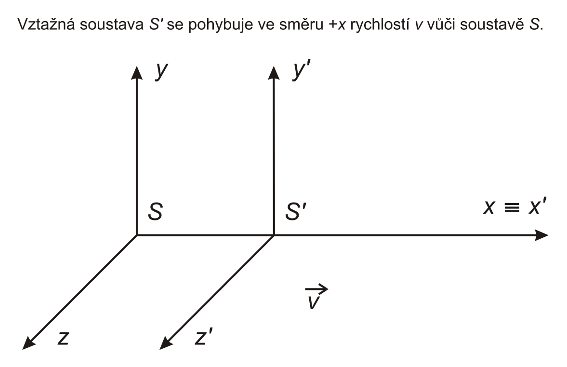
\includegraphics[width=0.5\textwidth]{vztazna_soustava}
\caption{Nákres vzájemné polohy vztažných soustav $ S $ a $ S^\prime $.}
\label{fig:vztazna_soustava}
\end{figure}
\[ x^\prime = \frac{x - vt}{\sqrt{(1 - \frac{v^2}{c^2})}} \]
\[ y^\prime = y \]
\[ z^\prime = z \]
\[ t^\prime = \frac{t - \frac{vx}{c^2}}{\sqrt{(1 - \frac{v^2}{c^2})}} \]
Pro zjednodušení zápisu se často zavádí bezrozměrná rychlost $ \beta $ a tzv. 
Lorentzův faktor $ \gamma $ vztahy:
\[ \beta \equiv {v\over c} \,, \]
\[ \gamma \equiv {1 \over \sqrt{1-\beta^2}} \,. \]
Počítáme-li navíc v přirozených jednotkách, kde $ c = 1 $, můžeme speciální 
Lorentzovu transformaci zapsat stručněji s důrazem na fyzikální význam:
\[x^\prime = \gamma\left(x - vt\right)\]
\[y^\prime = y\]
\[z^\prime = z\]
\[t^\prime = \gamma\left(t - {vx/{c^2}}\right)\]



\paragraph{Dilatace času} (čili roztažení, zpomalení času) je fyzikální jev pozorovaný u všech objektů, které vzhledem k pozorovateli
\textit{pohybují se velkou rychlostí} (důsledek zákonů speciální teorie relativity) nebo
jsou v \textit{silnějším gravitačním poli} (důsledek zákonů obecné teorie relativity).
V případě dvou pohybujících se pozorovatelů je dilatace času vzájemná, tedy oba dva vnímají hodiny toho druhého jako pomalejší. Naproti tomu u dilatace času gravitačním polem se pozorovatelé shodnou na tom, že hodiny s vyšším gravitačním potenciálem jsou pomalejší než hodiny s nižším potenciálem (dále od středu gravitace).
\paragraph{Kontrakce délek} (Lorentzova kontrakce nebo Lorentzova-FitzGeraldova kontrakce) je fyzikální jev, kterým se označuje změna (zkrácení) délky objektu, který se vzhledem k pozorovateli pohybuje, než kdyby byl objekt a pozorovatel vůči sobě v klidu.
Při malých rychlostech (ve srovnání s rychlostí světla) jsou změny zanedbatelné, proto jej lze v rámci klasické fyziky zanedbat. Speciální teorie relativity však již s tímto jevem počítá.
\paragraph{Časoprostorový interval}
Vzdálenost mezi dvěma událostmi v prostoročasu se označuje jako prostoročasová vzdálenost (interval).Časoprostor nebo prostoročas je fyzikální pojem z teorie relativity sjednocující prostor a čas do jednoho čtyřrozměrného objektu. Čas hraje roli čtvrtého rozměru a je oproti zbylým třem prostorovým rozměrům význačný (například tím, že v něm lze pohybovat jen jedním směrem). V obecné teorii relativity je časoprostor obecně zakřivený a má strukturu variety. Projevy zakřivení časoprostoru pozorujeme jako gravitaci.
\paragraph{Minkowského metrika}
\[ ds^2 = −c^2 dt^2+ dx^2 + dy^2 + dz^2\] 
\[ ds^2 = −c^2 dt^2 + dr^2 + r^2 d\Theta^2 + r^2 sin^2\Theta d\phi^2 \]
\paragraph{Schwarzschildův poloměr}
je charakteristická vzdálenost pro každou hmotnost. Je to poloměr koule, do které musí být veškerá hmota o dané hmotnosti stlačena, aby již žádná síla nemohla odvrátit její zhroucení do gravitační singularity. Tento termín se používá ve fyzice a astronomii, zejména v teoriích gravitace jako je napříklat Obecná teorie relativity.

\paragraph{Jak ovlivňuje gravitační pole chod času?}
vid dilatace casu.
\paragraph{Gravitační Dopplerův jev}
Podle obecné teorie relativity kolem sebe tělesa zakřivují prostor a čas. V pokřiveném časoprostoru se potom pohybují po nejrovnějších možných drahách, tzv. geodetikách. Jedním z důsledků zakřivení času v okolí hmotných těles je různý chod hodin v různé vzdálenosti od daného tělesa. Tento jev můžeme měřit buď přímo za pomoci hodin umístěných v různé vzdálenosti od tělesa (Země) nebo pomocí červeného gravitačního posuvu. Foton opouštějící hmotné těleso (například Zemi) v důsledku změny chodu času (a změny zakřivení prostoru) mění svou frekvenci a červená, tj. prodlužuje svou vlnovou délku, což je měřitelné.
\paragraph{Fridmanova metrika}
\[ ds^2 = – c^2 dt^2+ a^2(t) [ dr^2/(1 – kr^2) +  r^2d\omega^2 ] \]
\paragraph{Co vyjadřuje skalární křivost?}
Riemannův (Riemannův-Christoffelův) tenzor křivosti zachycuje v Riemannově geometrii křivost Riemannova prostoru. Riemannův tenzor křivosti lze použít k vyjádření křivosti libovolné variety s afinní konexí.

\paragraph{Co vyjadřuje expanzní funkce?}
\paragraph{Kosmologický posuv}
Spektrální čáry chemických prvků ve spektrech vzdálených objektů jsou proti měřením v pozemských chemických laboratořích posunuty směrem k dlouhovlnnému konci spektra. Tento rudý posuv spektrálních čar je tím větší, čím větší je vzdálenost pozorovaného objektu od Země a že i galaxie vzájemně se od sebe vzdalují rychlostí tím větší, čím jsou od sebe vzdálenější (Hubbleův zákon). To vede k teorii o rozpínání vesmíru.
\paragraph{Hubbleův zákon}
Pro rychlost vzdalování vzdáleného objektu $ v $  platí:
\[v = H_0D\]
kde\\
$ H_0 \approx 2.3 \cdot 10^{-18} s^{-1}$ je Hubbleova konstanta  a $ D $ je vzdialenost galaxie.

\paragraph{Hubbleův čas} je miera expanzie 
\[ \frac{1}{H_0}\]
\paragraph{Jak starý je vesmír?}
\end{document}
